In order to effectively transmit in the UHF TV band, it is mandatory to avoid interference with legacy users like wireless microphones, radio astronomy and existing TV channels. Wireless microphones are the ones that cause most of the problems when building a detector, mainly because of their narrow-band transmissions, low transmit power and (usually) unknown location. 

There are several techniques for determining the presence of signal in the UHF TV band, namely energy detection~\cite{cabric2006experimental}, cyclostationary detection~\cite{kim2007cyclostationary} and feature detection~\cite{cabric2006spectrum}. In this work, an energy detection approach is implemented due to its low complexity.

The proposed approach gathers the Power Spectral Density (PSD) of a set of samples taken every \emph{SampleSteps} (SS) Hertz in a determined frequency band. After the gathering, post-processing carries the task of identifying which power levels could be considered as noise based on the statistics of the sampled spectrum.

The identification of White Spaces is performed in a standalone USRP-E110 (see Figure~\ref{fig:usrp_combined}) using the WBX RX/TX Daughterboard~\cite{ettusWBX}, GNURadio~\cite{GNURadio} and a modified example code for spectrum sensing~\cite{sanabriaCodeUSRP} to account for different RF daughterboards and antennas. Figure~\ref{fig:connections} presents the connection layout between the USRP-E110 and a PC. This connection was used to transmit the executable code to the USRP and then to retrieve the White Spaces estimation file.

Both the PC and USRP-E110 belong to the same subnet and the communication was established inside a standard SSH tunnel.

\begin{figure}[htbp]
  \centering
  \includegraphics[width = 11cm]{sect2/figures/USRP_commented.eps}
  \caption{USRP-E110 external and internal overview. Equipped with WBX Daughterboard.}
  \label{fig:usrp_combined}
\end{figure}


\begin{figure}[htbp]
  \centering
  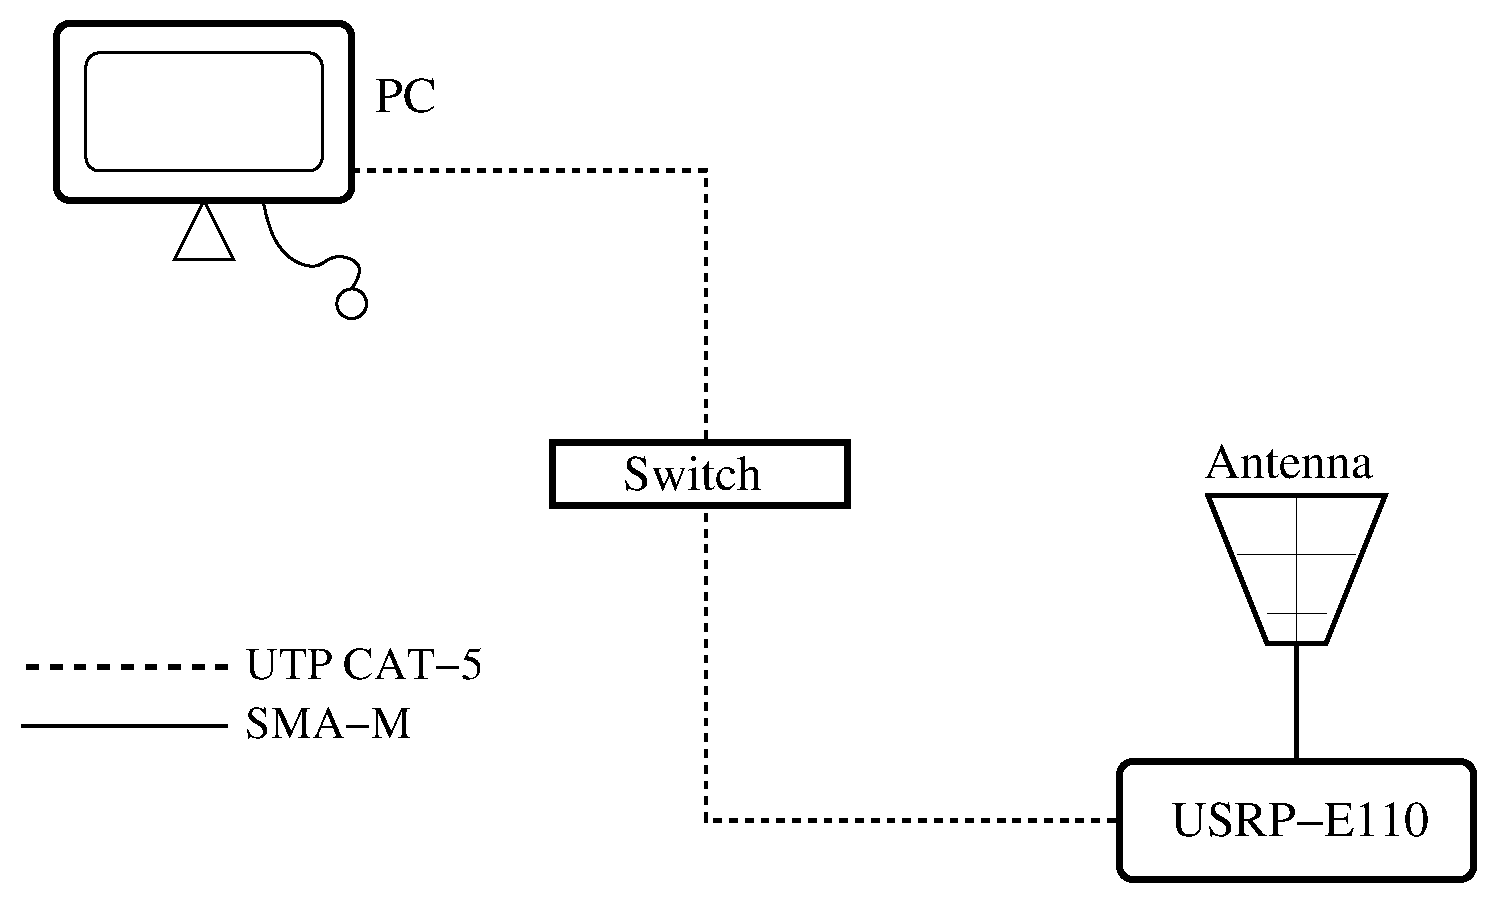
\includegraphics[width = 9cm]{sect2/figures/connections.eps}
  \caption{PC-USRP connections layout}
  \label{fig:connections}
\end{figure}